
\clearpage


\section{Preqin}
\label{sec:preqin}


% latex table generated in R 3.4.2 by xtable 1.8-4 package
% Wed Jul  1 13:54:55 2020
\begin{table}[ht]
	\centering
	\begin{tabular}{l@{\hskip 0.3in}l@{\hskip 0.2in}l@{\hskip 0.2in}l@{\hskip 0.2in}l@{\hskip 0.2in}l@{\hskip 0.1in}}
		Type & MKT-RF & HML & SMB & HDY-MKT & QLT-MKT \\ 
		\hline
		\hline
		BO & 1.33 (0.15) & -0.15 (0.12) & 0.2 (0.03) & 0.3 (0.1) & 0.21 (0.05) \\ 
		DD & 0.96 (0.09) & -0.11 (0.04) & 0.21 (0.01) & 0.14 (0.1) & 0.16 (0.05) \\ 
		%FOF & 1.22 (0.23) & -0.43 (0.09) & -0.24 (0.05) & -0.54 (0.09) & -0.01 (0.04) \\ 
		INF & 0.71 (0.22) & -0.37 (0.06) & -0.33 (0.13) & -0.47 (0.35) & 0.36 (0.11) \\ 
		MEZZ & 1.08 (0.13) & 0.06 (0.1) & 0.14 (0.04) & 0.16 (0.1) & 0.06 (0.11) \\ 
		NATRES & 0.36 (0.27) & -0.04 (0.22) & -0.02 (0.22) & 0.16 (0.36) & 0.11 (0.17) \\ 
		PD & 0.96 (0.08) & -0.07 (0.04) & 0.16 (0.03) & 0.06 (0.09) & 0.15 (0.04) \\ 
		%PE & 1.35 (0.16) & -0.2 (0.09) & 0.14 (0.07) & 0.24 (0.12) & 0.17 (0.04) \\ 
		RE & 1.14 (0.44) & -0.3 (0.16) & -0.42 (0.13) & -0.91 (0.15) & -0.4 (0.1) \\ 
		%SEC & 1.34 (0.25) & -0.36 (0.17) & -0.2 (0.07) & -0.29 (0.33) & 0.13 (0.04) \\ 
		VC & 1.02 (0.67) & -0.61 (0.11) & -0.42 (0.03) & -0.75 (0.14) & 0.84 (0.61) \\ 
		\hline
		MKT & 1 & 0 & 0 & 0 & 0 \\ 
		\hline
		\hline
	\end{tabular}
	\caption{
		PREQIN 2020: Multivariate five-factor models obtained by simple coefficient averaging (with standard deviations in parenthesis).
	} 
	\label{tab:average_coefs_preqin_2020}
\end{table}


% latex table generated in R 3.4.2 by xtable 1.8-4 package
% Fri Jul  3 14:50:53 2020
\begin{table}[ht]
	\centering
	\begin{tabular}{lrrrrr}
		Type & \multicolumn{4}{c}{Annualized Return} & Sharpe Ratio \\ 
		\cmidrule(r){2-5}
		& mean.R & stdv.R & mean.R-RF & stdv.R-RF & mean/stdv.R-RF \\ 
		\hline
		\hline
		BO & \textbf{0.152} & 0.195 & \textbf{0.125} & 0.196 & 0.641 \\ 
		DD & 0.116 & 0.144 & 0.091 & 0.144 & 0.630 \\ 
		%FOF & 0.120 & 0.200 & 0.094 & 0.200 & 0.470 \\ 
		INF & 0.085 & 0.119 & 0.060 & 0.119 & 0.506 \\ 
		MEZZ & 0.120 & 0.162 & 0.094 & 0.162 & 0.581 \\ 
		NATRES & 0.057 & \textbf{0.049} & 0.033 & \textbf{0.049} & \textbf{0.671} \\ 
		PD & 0.113 & 0.143 & 0.087 & 0.143 & 0.610 \\ 
		%PE & 0.151 & 0.200 & 0.125 & 0.200 & 0.624 \\ 
		RE & 0.092 & 0.203 & 0.067 & 0.203 & 0.329 \\ 
		%SEC & 0.137 & 0.207 & 0.111 & 0.207 & 0.537 \\ 
		VC & 0.124 & 0.176 & 0.099 & 0.176 & 0.561 \\ 
		\hline
		MKT & 0.107 & 0.152 & 0.082 & 0.152 & 0.536 \\ 
		\hline
		\hline
	\end{tabular}
	\caption{
		PREQIN 2020: 
		Annualized average returns, standard deviations (annualized by the square root of time formula), and Sharpe ratios (i.e., the ratio of mean.R-RF to stdv.R-RF) implied by the five-factor models from table \ref{tab:average_coefs_preqin_2020}. 
		The underlying monthly returns are based on MSCI World style indices (in USD) from 1996-01-31 to 2020-05-31.
	} 
	\label{tab:ann_returns_preqin_2020}
\end{table}


\begin{figure}[H]
	\centering
	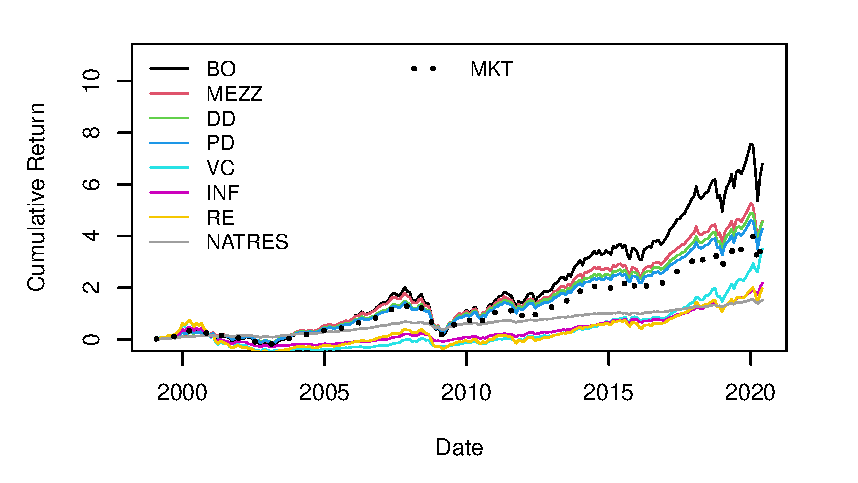
\includegraphics{Figures/Cumulative_Returns_2020.eps}
	\caption{
		PREQIN 2023: Cumulative USD returns implied by the MSCI World factor models from Table \ref{tab:average_coefs_preqin_2020} from 1999-01-31 until 2023-02-28.}
	\label{fig:cum_returns_preqin}   
\end{figure}



% latex table generated in R 3.6.1 by xtable 1.8-4 package
% Tue Jul 28 12:13:36 2020
\begin{table}[ht]
	\centering
	\begin{tabular}{lrrrrrrrr}
		Vintage & BO & DD & INF & MEZZ & NATRES & PD & RE & VC \\ 
		\hline
		\hline
		%1983 &   0 &   0 &   0 &   0 &   0 &   0 &   0 &   0 \\ 
		1984 &   0 &   0 &   0 &   0 &   0 &   0 &   0 &   1 \\ 
		1985 &   3 &   0 &   0 &   0 &   0 &   0 &   0 &   4 \\ 
		1986 &   2 &   0 &   0 &   1 &   0 &   1 &   0 &   4 \\ 
		1987 &   4 &   0 &   0 &   1 &   0 &   1 &   0 &   3 \\ 
		1988 &   7 &   0 &   0 &   0 &   0 &   0 &   0 &   2 \\ 
		1989 &   2 &   0 &   0 &   0 &   1 &   0 &   0 &   2 \\ 
		1990 &   5 &   1 &   0 &   0 &   0 &   1 &   0 &   6 \\ 
		1991 &   3 &   2 &   0 &   0 &   0 &   2 &   0 &   4 \\ 
		1992 &   9 &   2 &   0 &   2 &   1 &   4 &   1 &   7 \\ 
		1993 &   7 &   0 &   0 &   0 &   0 &   0 &   0 &   4 \\ 
		1994 &   9 &   1 &   0 &   2 &   1 &   3 &   1 &   7 \\ 
		1995 &  17 &   0 &   0 &   1 &   1 &   1 &   1 &  10 \\ 
		1996 &  16 &   2 &   0 &   2 &   0 &   4 &   4 &  10 \\ 
		1997 &  16 &   2 &   0 &   0 &   1 &   2 &   6 &  14 \\ 
		1998 &  30 &   1 &   0 &   3 &   2 &   4 &   3 &  23 \\ 
		1999 &  28 &   1 &   0 &   7 &   1 &   8 &   2 &  37 \\ 
		2000 &  32 &   3 &   0 &   4 &   0 &   7 &   6 &  67 \\ 
		2001 &  18 &   2 &   0 &   3 &   1 &   5 &   2 &  40 \\ 
		2002 &  24 &   4 &   1 &   2 &   2 &   6 &   2 &  24 \\ 
		2003 &  18 &   3 &   1 &   2 &   1 &   5 &   6 &  19 \\ 
		2004 &  29 &   2 &   4 &   3 &   2 &   5 &  10 &  29 \\ 
		2005 &  63 &   6 &   0 &   7 &   4 &  14 &  19 &  34 \\ 
		2006 &  76 &  10 &   5 &   5 &   3 &  16 &  34 &  41 \\ 
		2007 &  88 &  13 &   5 &   3 &   7 &  16 &  36 &  53 \\ 
		2008 &  76 &  12 &   3 &   6 &   8 &  21 &  35 &  40 \\ 
		2009 &  35 &   7 &   5 &   4 &   4 &  12 &  14 &  20 \\ 
		2010 &  53 &   9 &   9 &   7 &   8 &  18 &  40 &  21 \\ 
		2011 &  72 &   8 &  11 &   6 &   9 &  16 &  51 &  27 \\ 
		2012 &  69 &  14 &   4 &  11 &  11 &  26 &  42 &  25 \\ 
		2013 &  80 &  15 &  12 &   4 &   8 &  32 &  61 &  30 \\ 
		2014 &  88 &  13 &  12 &   5 &  15 &  31 &  56 &  36 \\ 
		2015 &  99 &  18 &  13 &   7 &   9 &  38 &  86 &  47 \\ 
		2016 & 108 &   8 &  16 &   8 &  16 &  29 &  63 &  56 \\ 
		2017 &  83 &  15 &  20 &   8 &  13 &  48 &  78 &  56 \\ 
		2018 &  88 &  22 &  18 &  11 &   8 &  54 &  71 &  55 \\ 
		2019 &  21 &   3 &   5 &   2 &   1 &  11 &  12 &  11 \\ 
		\hline
		Total & 1378 & 199 & 144 & 127 & 138 & 441 & 742 & 869 \\ 
		\hline
		\hline
	\end{tabular}
	\caption{PREQIN 2020: Number of funds per vintage year in the Preqin dataset used for estimation (Preqin cash flow data set as of 26th February 2020).} 
	\label{tab:preqin_data}
\end{table}


\newpage


% Factor Model Returns + Errors
\renewcommand{\segment}{PE}

\subsection{Preqin: Idiosyncratic returns for \segment \ funds}
\label{sec:preqin_errors_\segment}

\begin{figure}[H]
	\centering
	\includegraphics{Figures/q_factors/XErrorSeries\segment Preqin}
	\caption{Idiosyncratic returns estimated by componentwise $L_2$ boosting for fund type \segment \ in the period from 1990-03-31 until 2019-09-30.}
	\label{fig:preqin_clb_idio_\segment}
\end{figure}

\begin{figure}[H]
	\centering
	\includegraphics{Figures/q_factors/XTotalErrorSeries\segment Preqin}
	\caption{
		Comparison between the total returns for fund type \segment \ implied by our two-factor ensemble and our two-factor ensemble plus the error term from Figure \ref{fig:preqin_clb_idio_\segment}.
		Both series are contrasted against the NAV Return indices provided by Cambridge Associates and Pitchbook and the MSCI stock market index in the period 1990-03-31 until 2019-09-30.
	}
	\label{fig:preqin_clb_total_\segment}
\end{figure}

\begin{figure}[H]
	\centering
	\includegraphics{Figures/q_factors/XTotalErrorSeries\segment Preqinpre2010}
	\includegraphics{Figures/q_factors/XTotalErrorSeries\segment Preqinpost2010}
	\caption{
		In these two subplots, we split the full \segment \ time series from Figure \ref{fig:preqin_clb_total_\segment} into a pre-2010 and post-2010 period.
	}
	\label{fig:preqin_clb_pre_post_2010_\segment}
\end{figure}


% Factor Model Returns + Errors
\renewcommand{\segment}{VC}

\subsection{Preqin: Idiosyncratic returns for \segment \ funds}
\label{sec:preqin_errors_\segment}

\begin{figure}[H]
	\centering
	\includegraphics{Figures/q_factors/XErrorSeries\segment Preqin}
	\caption{Idiosyncratic returns estimated by componentwise $L_2$ boosting for fund type \segment \ in the period from 1990-03-31 until 2019-09-30.}
	\label{fig:preqin_clb_idio_\segment}
\end{figure}

\begin{figure}[H]
	\centering
	\includegraphics{Figures/q_factors/XTotalErrorSeries\segment Preqin}
	\caption{
		Comparison between the total returns for fund type \segment \ implied by our two-factor ensemble and our two-factor ensemble plus the error term from Figure \ref{fig:preqin_clb_idio_\segment}.
		Both series are contrasted against the NAV Return indices provided by Cambridge Associates and Pitchbook and the MSCI stock market index in the period 1990-03-31 until 2019-09-30.
	}
	\label{fig:preqin_clb_total_\segment}
\end{figure}

\begin{figure}[H]
	\centering
	\includegraphics{Figures/q_factors/XTotalErrorSeries\segment Preqinpre2010}
	\includegraphics{Figures/q_factors/XTotalErrorSeries\segment Preqinpost2010}
	\caption{
		In these two subplots, we split the full \segment \ time series from Figure \ref{fig:preqin_clb_total_\segment} into a pre-2010 and post-2010 period.
	}
	\label{fig:preqin_clb_pre_post_2010_\segment}
\end{figure}



% Factor Model Returns + Errors
\renewcommand{\segment}{RE}

\subsection{Preqin: Idiosyncratic returns for \segment \ funds}
\label{sec:preqin_errors_\segment}

\begin{figure}[H]
	\centering
	\includegraphics{Figures/q_factors/XErrorSeries\segment Preqin}
	\caption{Idiosyncratic returns estimated by componentwise $L_2$ boosting for fund type \segment \ in the period from 1992-06-30 until 2019-09-30.}
	\label{fig:preqin_clb_idio_\segment}
\end{figure}

\begin{figure}[H]
	\centering
	\includegraphics{Figures/q_factors/XTotalErrorSeries\segment Preqin}
	\caption{
		Comparison between the total returns for fund type \segment \ implied by our two-factor ensemble and our two-factor ensemble plus the error term from Figure \ref{fig:preqin_clb_idio_\segment}.
		Both series are contrasted against the NAV Return indices provided by Cambridge Associates and Pitchbook and the MSCI stock market index in the period 1990-03-31 until 2019-09-30.
	}
	\label{fig:preqin_clb_total_\segment}
\end{figure}

\begin{figure}[H]
	\centering
	\includegraphics{Figures/q_factors/XTotalErrorSeries\segment Preqinpre2010}
	\includegraphics{Figures/q_factors/XTotalErrorSeries\segment Preqinpost2010}
	\caption{
		In these two subplots, we split the full \segment \ time series from Figure \ref{fig:preqin_clb_total_\segment} into a pre-2010 and post-2010 period.
	}
	\label{fig:preqin_clb_pre_post_2010_\segment}
\end{figure}

